\documentclass{article}
\usepackage{hyperref}
\usepackage{epsfig}

\author{Hannes Mehnert\\IT University of Copenhagen\\\texttt{hame@itu.dk}}
\title{Design and Implementation of Kopitiam}

\begin{document}
\maketitle

\section{Introduction}
We are developing Kopitiam, a plugin for Eclipse to interactively prove correctness of Java programs using separation logic by interacting with the theorem prover Coq. Proofs are developed side-by-side with the Java program in Eclipse, allowing seamless integration into the normal developers workflow.

Kopitiam is written in Scala, a type-safe class-based functional object-oriented language supporting pattern matching which compiles to Java bytecode. Thus, Scala programs can easily interface to Java code.

This document describes the design of Kopitiam: we give an overview of Kopitiam in section \ref{section:overview}, afterwards describe the interaction with Coq in section \ref{section:coq}, the unified representation of Coq proofs and Java code in section \ref{section:representation}, the extensions to Eclipse in section \ref{section:eclipse} and finally the desirable improvements in section \ref{section:improvements}. In section \ref{section:scala} we give a brief overview of Scala, if you are not familiar with Scala we recommend that you read that section first.

\section{Overview of Kopitiam} \label{section:overview}
Kopitiam consists of multiple parts communicating with other tools. Figure \ref{fig:kop-over} shows the communication overview, Java source code with specifications (pre- and postconditions) and Coq proofs are interactively developed in Eclipse, while Coq is run in a separate process to do the proofs. All interaction is encoded using UTF-8. The Java source including specifications is stored in files, communication happens with Eclipse via the plugin interface and with Coq via standard input and output.

\begin{figure}
\centering
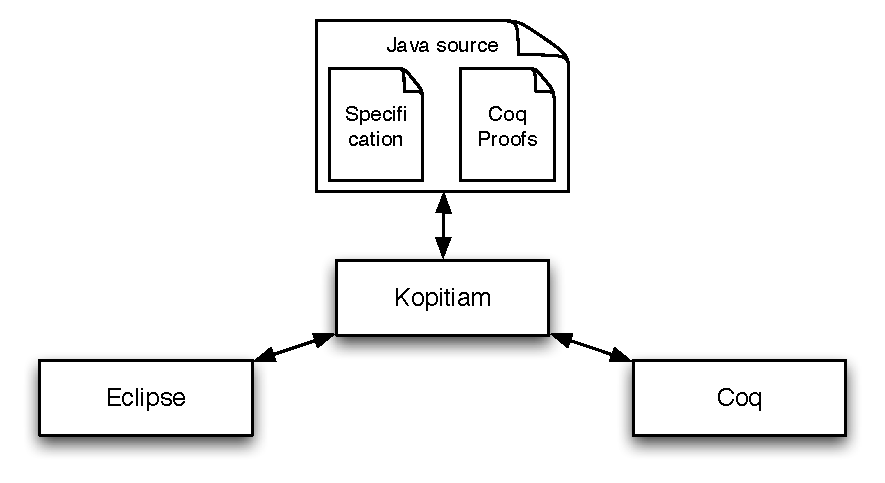
\epsfig{file=kopitiam-overview, scale=0.6}
\caption{Kopitiam input/output overview}
\label{fig:kop-over}
\end{figure}

The provided, enriched Java code is still valid Java code, which can be compiled with a standard Java compiler. It contains the preconditions, postconditions and Coq proofs as calls to static methods of a stub class. Our research group developed a semantics for SimpleJava \ref{subsection:simplejava} in Coq, together with an assertion logic, a specification logic and proof tactics.

\section{Coq interaction} \label{section:coq}
Two different approaches are imaginable for interaction with Coq: either (a) directly call methods of Coq or (b) run the command-line binary (called \texttt{coqtop}) in a separate process and interact via console standard input and output (stdin/stdout).

In approach (a) the data structures of Coq could be reused, whereas in (b) the string representation, intended for human consumption rather than for a machine, has to be parsed. But we haven't found a way to interface OCaml code into JVM bytecode. The only way we discovered is to run from OCaml exported C code via the Java Native Interface (JNI). Using this \url{http://ocamljava.x9c.fr/}, type information is lost and interfaces have to be developed both on Java and on OCaml side.

We chose (b), that is, to run \texttt{coqtop} as a separate process and connect a Scala actor to stdout and stderr. This is also the approach taken by \texttt{ProofGeneral}, the Emacs interface of Coq. The argument \texttt{-emacs} to \texttt{coqtop} changes its behavior, it then provides a more machine-readable output, including step-numbers and the set of current theorems. The interactive shell of \texttt{coqtop} is sent on stderr, while error messages and other informational messages are sent to stdout.

In Kopitiam, a Scala singleton CoqTop is a wrapper around the \texttt{coqtop} binary, providing start and setup of Coq (method \texttt{startCoq()}), which installs BusyStreamReader on stdout and stderr. The singleton CoqTop also provides input handling for Coq, a method which waits until Coq is ready for input and then writes a string (method \texttt{writeToCoq(data : String)}). There are also methods which keep track whether \texttt{coqtop} has been started (method \texttt{isStarted() : Boolean}) or is currently busy (method \texttt{isReady() : Boolean}).

The in Kopitiam defined class BusyStreamReader reads, in a busy loop, all data from the given stream. It sends received data to every registered actor.

The in Kopitiam defined singleton ErrorOutputActor is registered at the BusyStreamReader which reads from the stderr of \texttt{coqtop} and parses the interactive Coq shell. It uses the singleton ValidCoqShell, which is a hand-written parser (in Kopitiam), which checks that global and local steps are increasing and the same theorem as the previous is in context. The singleton ErrorOutputActor then either does a call to commit or an undo on the singleton DocumentState (also defined in Kopitiam). The context, consisting of theorems and steps, is preserved in a local variable (it's type is CoqShellTokens) for the next sanity check. TODO: this DocumentState should be local to every open CoqDocument

The in Kopitiam defined singleton PrintActor is registered at the BusyStreamReader which reads from the stdout of \texttt{coqtop} and uses the CoqResponseParser combinator parser (developed in Kopitiam) to categorize the received answer, which must be a case class of trait CoqResponse (also defined in Kopitiam). The PrintActor then sends the parsed answer to all registered CoqCallback (a trait defined in Kopitiam), by calling the method \texttt{dispatch(x : CoqResponse)} on each of them. The purpose of categorization is to distinguish between error messages (case class CoqError), achieved goals (case class CoqTheoremDefined and CoqProofCompleted) and proof obligations (case class CoqGoal), and have separate handlers for these.

To print error messages on the external class Console (Java system library) or EclipseConsole (provided by Eclipse) in the singleton PrintActor, the alias type Printable is defined, which can be any object providing a method \texttt{println(s : String)}. This is in place to use the Coq interaction with and without Eclipse (the external classes EclipseConsole and Console have no common superclass apart from Object).

\section{Unified Coq and Java representation} \label{section:representation}
We developed a single representation of Java source code, specification and Coq proofs, together with input and output facilities, shown in Figure \ref{fig:repr}, which is a zoom into the interaction between source files and Kopitiam of Figure \ref{fig:kop-over}. The central part of Kopitiam is the unified representation, which are instances of the JStatement trait, stored in the singleton ClassTable. The input for this unified representation is either Java source code, which is parsed by the JavaParser trait, then transformed to SimpleJava (see Subsection \ref{subsection:simplejava}) by the traits FinishAST and JavaToSimpleJava. The other input possibility is Coq source, which is parsed and translated by the CoqParser trait. There are two different outputs for the unified representation, either using the JavaOutputter to generate SimpleJava source code, which is a subset of Java and thus can be compiled by any Java compiler or using the CoqOutputter to generate Coq source code, which can be passed to Coq.

\begin{figure}
\centering
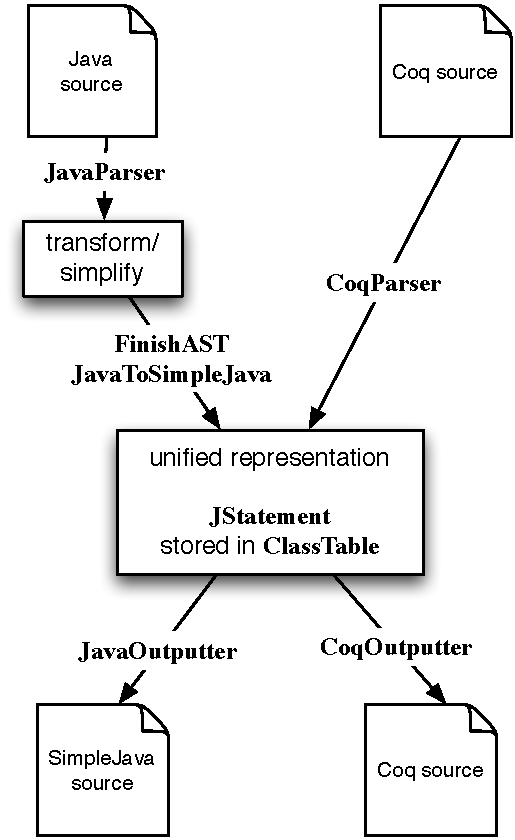
\epsfig{file=kopitiam-representation, scale=0.6}
\caption{Kopitiam's unified representation and its input and output facilities}
\label{fig:repr}
\end{figure}

The standard usage of the tool is to start developing a Java program, adding pre- and postconditions, develop a mathematical model in the Coq editor and then interactively discharge the proof obligations. The Java source code is immediately translated into Coq. The Coq proofs are immediately translated into Java source. Thus, the single unified representation is always in sync with outputs and inputs. (TODO: Coq parser is currently not connected to this feedback loop)

The Java combinator parser integrated in Kopitiam is based on Paul Philipps Java parser, available on github \footnote{\url{https://github.com/paulp/scala-lang-combinators/tree/master/src-java}}. We forked his work and continue development in the dk.itu.sdg.javaparser package.

The lexer, implemented in class JavaLexer, treats string literals specially by already transform \textbackslash" to ".

Parser combinators for Java expressions are defined in the Expression trait, statements are parsed by the JavaParser trait (unclear why there is this distinction), both produce instances of the original intermediate language, defined in the trait JavaTerms. This original intermediate language has only weak types, several fields have the type Any, several fields use an Option[Any] type. This representation is convenient for writing the parser combinators (where due to no left recursion etc. some parse rules parse partial statements or expressions). But later it is more convenient to work with an intermediate language which is more precisely typed (and thus allows fewer inconsistencies). We developed this second intermediate language with the trait JStatement, and the trait FinishAST transforms a JavaTerm representation to a JStatement representation.

In contrast to Java, SimpleJava does not contain inner classes, fewer operators, only a single return statement and restricts field access to statements instead of expressions. Java can be transformed to SimpleJava, we implemented this transformation in the trait JavaToSimpleJava. For this transformation we collect some semantic information (types of local variables, fields,...) in FinishAST. In the trait JavaToSimpleJava this information is analyzed and temporary variables are introduced on demand (method \texttt{extractCalls}). The trait FinishAST (TODO: why is that in there?) moves inner classes to the top level, preserving the information of the outer class, so field accesses to the outer class are handled properly. Java's visibility information is discarded, because it is not needed in SimpleJava.

TODO: formalize extractCalls and innerClass to top-level

We implemented two pretty printers, CoqOutputter and JavaOutputter. The CoqOutputter prints Coq code, including separation of specification and code in different modules, as required by our formalization in Coq. It also generates the boilerplate in Coq of defining proper Program and Class definitions. The JavaOutputter prints Java code, including specification and Coq proofs as calls to static methods of a stub Coq class.

TODO: In the package dk.itu.sdg.coqparser we implemented a lexer and parser for Coq, which translates Coq source into JStatement intermediate representation.


\subsection{SimpleJava} \label{subsection:simplejava}
The grammar of SimpleJava is shown in Figure \ref{fig:simplejava}. A Program consists of any number of class and interface definitions. An interface definition consists of a name, a list of extended interfaces and a list of method signatures. A class definition consists of a name, a list of implemented interfaces, a list of fields and a list of methods. Each method has a signature, including a return type and a list of arguments (each is a pair of name and type). A method body consists of a sequence of statements, either read or write field access, assignment, call, allocation, a loop or a conditional. Expressions are either arithmetic or boolean expressions or variable access or a literal constant. The last statement of a method body must be a return statement, returning a single expression.

\begin{figure}
\texttt{P ::= C | I}\\
\texttt{I ::= interface I extends $\overline{I}$ \{ $\overline{MSig}$ \}}\\
\texttt{C ::= class C implements $\overline{I}$ \{ $\overline{F}$ ; $\overline{M}$ \}}\\
\texttt{F ::= type field}\\
\texttt{MSig ::= type method n ($\overline{e}$)}\\
\texttt{M ::= type method n ($\overline{e}$) \{ $\overline{c}$; return x \}}\\
\texttt{c ::= x := e.f | e.f := x | x := e | y := x.m($\overline{e}$) | x := alloc C | while e do \{ $\overline{c}$ \} | if e then $\overline{c}$ else $\overline{c}$}\\
\texttt{e ::= e1 aop e2 | e1 bop e2 | ! b | var | constant}\\
\texttt{aop ::= + | * | -}\\
\texttt{bop ::= \& | |}\\
\texttt{type ::= boolean | int | C}\\
\caption{SimpleJava grammar}
\label{fig:simplejava}
\end{figure}

\section{Eclipse integration} \label{section:eclipse}
The integration of Kopitiam into Eclipse (in package dk.itu.sdg.kopitiam) provides the possibility to develop code and proofs side-by-side. This is shown in Figure \ref{fig:coqjava}, where on the left the Java code is developed in a standard JavaEditor (provided by Eclipse), while on the right the correctness proof is developed (in a CoqEditor, a part of Kopitiam). In Figure \ref{fig:goal}, the GoalViewer is shown (also a part of Kopitiam), which displays the current proof obligation.

\begin{figure}
\centering
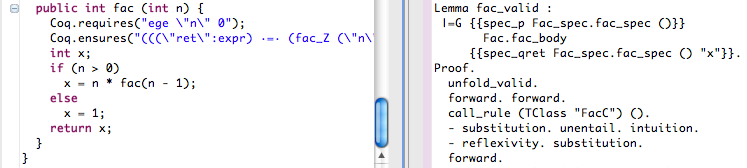
\epsfig{file=coqjava, scale=0.6}
\caption{Coq and Java editor, side-by-side}
\label{fig:coqjava}
\end{figure}

\begin{figure}
\centering
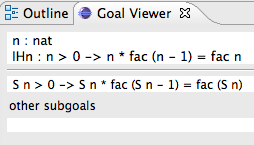
\epsfig{file=goal-buffer, scale=0.5}
\caption{Kopitiam's GoalViewer}
\label{fig:goal}
\end{figure}


Eclipse provides extension points to facilitate extensions by a plugin. Kopitiam extends Eclipse with CoqEditor, an editor for Coq. It uses a custom IDocumentProvider (called CoqJavaDocumentProvider), which translates any Java source including specifications and proofs to Coq, using the JavaParser mentioned in the previous section. A global map from Java files to CoqDocument objects (a subclass of Eclipse's Document containing the string representation generated by CoqOutputter, which was described in the previous section) is stored by Kopitiam in the object EclipseTables to apply changes in one of the files to the other. The CoqJavaDocumentProvider also has the facility to update parts of a document (method \texttt{up}) by calling the method \texttt{update} implemented in FinishAST. This parses the whole Java document and returns the offset and length of the first changed method of the first class. TODO: this is a hardcoded hack for presentation, should be general that it parses only the part needed and updates only that part

The singleton object DocumentState marks the current position (field position) of the file which Coq is interacting with as well as the length of the command in progress (field sendlen). It provides two methods, \texttt{undo}, which reverts the string of the last sent command in the CoqEditor to black, and \texttt{commit}, which marks the string of the command blue. These methods are called by the ErrorOutputActor described in the previous section. TODO: should be a DocumentState for every CoqDocument

Another singleton object implemented in Kopitiam is EclipseBoilerPlate which provides the method \texttt{getContent} to get the content of the current active editor as string, the method \texttt{getResource} to get the IFile object of the current active editor and the method \texttt{mark}, which creates an Eclipse warning marker at the current position (taken from DocumentState). TODO: should use fewer global state

The GoalViewer shows the current state of the Coq proof, similar to the goal buffer in ProofGeneral. There are two buttons with connected actions, CoqStepAction and CoqUndoAction, provided by Kopitiam. CoqStepAction sends the command from the current Coq marker until the next '.' to Coq, CoqUndoAction sends an undo command to Coq. If the sent command is acknowledged by Coq, it is highlighted in the CoqEditor. TODO: too much global state

The singleton object CoqOutputDispatcher is registered at the PrintActor (described in section \ref{section:coq}) and handles the (stdout) output of Coq. It either creates an Eclipse warning, if a CoqError is reported by Coq (by using EclipseBoilerPlate) or writes proof obligations into the GoalViewer widget.

A naive IContentAssistantProcessor implementation (named CoqContentAssistantProcessor) provides some completion for Coq, currently a static list of tactics. It does not use any information of the current context (like proof state or defined variables).

The singleton object DocumentMonitor connects to all open editors and editors which will be opened in the future, by also registering as a listener for new Eclipse parts. It enables to track changes to any text file, propagating these to the model (and possibly to other views of the same model). It registers to all open windows by using Eclipse's IStartup extension point.

The single Java class, Activator, provides the \texttt{earlyStartup} method required by the IStartup interface, and is mainly present to find needed imports in Eclipse, which might be cumbersome manually.

\section{Desirable Improvements} \label{section:improvements}

\begin{itemize}
\item General
\begin{itemize}
\item remove the introduced global state - DocumentState - plus everything that depends on that
\item keep it simple, only one connection to a Coq binary
\item remove hack that first method of first class is in update
\item future: incrementally run proofer in the background, annoy user then with unproven stuff (when code is changed)
\end{itemize}
\item Coq side
\begin{itemize}
\item sometimes subgoals are only partially received, leading to CoqUnknown and partial/no display of subgoals (CoqTop/CoqResponse)
\item Outline in eclipse
\item syntax highlighting based on coq parser
\item debug coq parser
\item remove hack that searches for '. ' to send command
\item remove warning if it's void (specific source location has changed)
\item disable undo if no undo possible
\item retract proof/leave for later
\end{itemize}
\item Java side
\begin{itemize}
\item loop invariants
\item proper syntax (not only a string) for pre/postcondition and loop invariants - plus completion!
\item for loops
\item foo.bar.baz() doesn't work properly (need to introduce multiple temporary variables)
\item error on multiple returns and overloading of the same method name
\item return type of java methods from java standard library
\item field initializers
\item multiple local variables and fields: int foo, bar, baz
\end{itemize}
\item Java features
\begin{itemize}
\item Generics
\item Exceptions
\item array types
\end{itemize}
\end{itemize}

\section{Scala Overview} \label{section:scala}
Scala integrates several advanced programming language features directly in the language, the important ones are briefly described here:
\begin{itemize}
\item \textbf{Singleton} - A class which exists only once at runtime, this design pattern is integrated into the programming language (by using \texttt{object} instead of \texttt{class}).
\item \textbf{Immutability} - Bindings can be introduced with either \texttt{var} or \texttt{val}, the latter introduces an immutable binding. 
\item \textbf{Actor} - The primary concurrency construct in Scala is an actor, which is a sequential process that communicates by exchanging messages.
\item \textbf{Trait, Multiple Inheritance} - In addition to classes, traits are available. These are similar to interfaces in Java, but allow partial implementation. In contrast to classes, traits may not have constructor arguments and can't be instantiated, thus a trait is similar to an abstract class. A class may extend multiple traits. A linearization algorithm is provided to linearize the inheritance DAG, which may contain diamonds, to a list.
\item \textbf{Higher-order} - Scala is higher-order, thus methods can be passed around as arguments to other methods. This allows functional programming and compact code (list comprehension etc.). This is also a crucial feature for the actors and pattern matching implementation, using partial functions.
\item \textbf{Subtyping} - The type system uses nominal subtyping, but structural subtyping is also supported if the developer needs it, he can use it explicitly.
\item \textbf{Implicit, Variance, Higher-order kinds} - Scala provides type variables with variance and implicits, which is at least as powerful as Haskell type classes.
\end{itemize}
%ref expression problem

\end{document}